\def\layersep{2.5cm}

\begin{figure}[H]
    \centering
    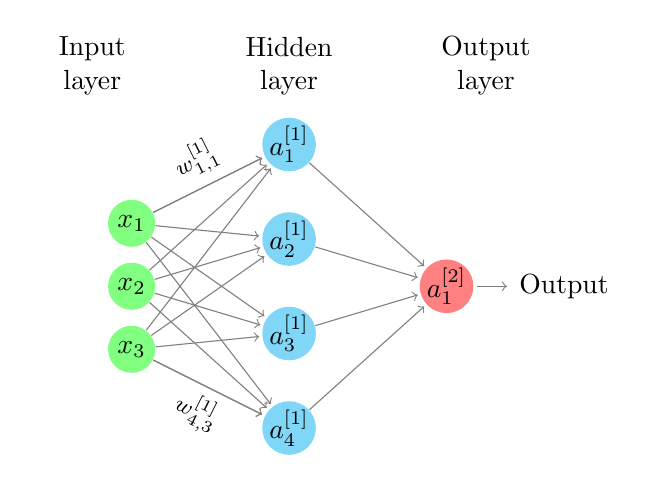
\begin{tikzpicture}[shorten >=1pt,->,draw=black!50, node distance=\layersep, scale=.8]
        \tikzstyle{every pin edge}=[<-,shorten <=1pt]
        \tikzstyle{neuron}=[circle,fill=black!25,minimum size=17pt,inner sep=0pt]
        \tikzstyle{input neuron}=[neuron, fill=green!50];
        \tikzstyle{output neuron}=[neuron, fill=red!50];
        \tikzstyle{hidden neuron}=[neuron, fill=cyan!50];
        \tikzstyle{annot} = [text width=4em, text centered]
        
        % Draw the input layer nodes
        \foreach \y in {1,...,3} {
            \node[input neuron] (I-\y) at (0,{1 -(\y - 1)}) {$x_{\y}$};
        }
        % Draw the hidden layer nodes
        \foreach \y in {1,...,4} {
            \node[hidden neuron] (H-\y) at (\layersep,{2.25 - 1.5*(\y -1)}) {$a^{[1]}_{\y}$};
        }
        
        % Draw the output layer node
        \node[output neuron,pin={[pin edge={->}]right:Output}] (O) at ({2*\layersep, 0}) {$a^{[2]}_1$};
        
        % Connect every node in the input layer with every node in the
        % hidden layer.
        \foreach \source in {1,...,3}
            \foreach \dest in {1,...,4}
                \path (I-\source) edge (H-\dest);
        
        \path (I-1) edge node[sloped, above] {\footnotesize  $w_{1, 1}^{[1]}$} (H-1);
        \path (I-3) edge node[sloped, below] {\footnotesize  $w_{4, 3}^{[1]}$} (H-4);
        
        % Connect every node in the hidden layer with the output layer
        \foreach \source in {1,...,4}
            \path (H-\source) edge (O);
        
        % Annotate the layers
        \node[annot,above of=H-1, node distance=1cm] (hl) {Hidden layer};
        \node[annot,left of=hl] {Input layer};
        \node[annot,right of=hl] {Output layer};
    \end{tikzpicture}
    \caption{Representation of Neural Network}
\end{figure}
